\chapter{Datasets and Evaluation}
\label{chap:testing}
This chapter describes the methods and databases used to gather data and evaluate the developed work. It also presents the \gls{ImageCLEF} competition to which the work will be submitted to.

\section{Common Sense Databases}
There are several databases that can be used to represent common sense for human reasonning.
From those databases several probabilistic relations can be derived in order to increase the quality of the model the robot uses for reasoning at high-level.
Examples of those databases are:

{OpenMind Common Sense}~\citep{singh2010open} which contains several sentence-templates filled in by humans by creating meaningful sentences (\autoref{fig:openmind-sample}). With those its possible to extract knowledge of finding certain objects in room categories.

\begin{figure}[!h]
\centering
\fbox{
\begin{minipage}{13 cm}
A kitchen floor is dirty when a kitchen floor is sticky.\\
A room where you generally find a muffin is the kitchen.\\
You generally find a blender in a kitchen.\\
An object that you might find in an office is a answering machine.\\
An object that you might find in an office is a briefcase.
\end{minipage}
}
\caption{Examples of sentences available on OpenMind Indoor Common Sense}
\label{fig:openmind-sample}
\end{figure}


\begin{figure}[!h]
\begin{center}
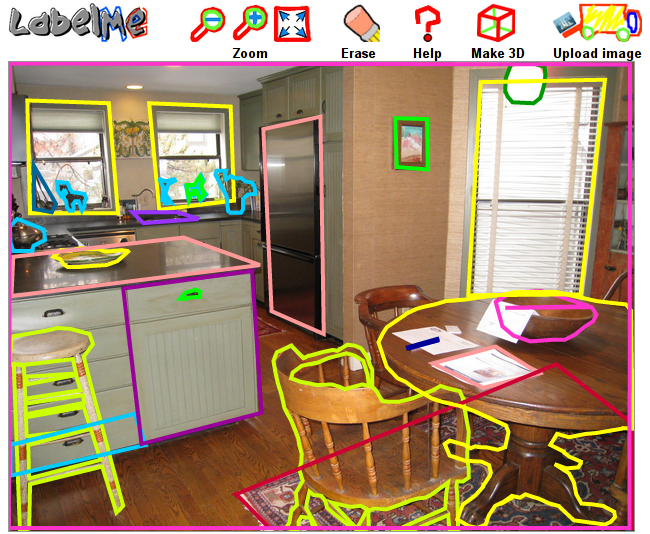
\includegraphics[width=0.7\textwidth]{labelme_kitchen_sample}
\end{center}
\caption{Sample annotated image from the LabelMe online database.}
\label{fig:labelme_sample}
\end{figure}

LabelMe~\citep{russell2008labelme} which is an online database for image annotation (\autoref{fig:labelme_sample}.
At the moment it counts with hundreds of thousands labelled objects.
There is both images and sequences of images that have been annotated.
The annotation does not only goes for objects but also for scene categories,
turning this database useful for extraction of data related with probabilities of finding objects in room categories. As well their appearance.

\section{Evaluation Databases}\label{sec:databases}
In order to train and evaluate the system real databases are required. In that sense we point to a previously used database: \gls{COLD}~\citep{pronobis09ijrr-cold}.

It contains image sequences captured using a regular and omni-directional cameras together with laser range scans and odometry data.
The data were recorded using three different mobile robot platforms and the same camera setup, under various weather and illumination conditions (during cloudy weather, sunny weather and at night) over several days.
In each of the three labs, the acquisition was performed in several rooms of different functionality.


\begin{figure}[!h]
\label{fig:cold-database-sample}
\begin{center}
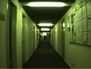
\includegraphics[width=0.15\textwidth]{cold/Saarbruecken_CR}
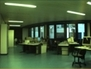
\includegraphics[width=0.15\textwidth]{cold/Saarbruecken_TR}
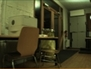
\includegraphics[width=0.15\textwidth]{cold/Freiburg_PA}
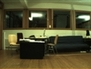
\includegraphics[width=0.15\textwidth]{cold/Freiburg_LO}
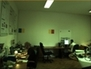
\includegraphics[width=0.15\textwidth]{cold/Ljubljana_LAB}
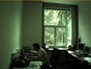
\includegraphics[width=0.15\textwidth]{cold/Ljubljana_2PO}

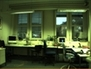
\includegraphics[width=0.15\textwidth]{cold/Saarbruecken_RL}
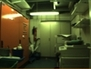
\includegraphics[width=0.15\textwidth]{cold/Saarbruecken_PA}
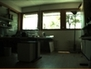
\includegraphics[width=0.15\textwidth]{cold/Freiburg_1PO}
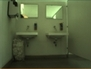
\includegraphics[width=0.15\textwidth]{cold/Freiburg_TL}
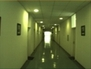
\includegraphics[width=0.15\textwidth]{cold/Ljubljana_CR}
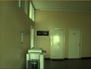
\includegraphics[width=0.15\textwidth]{cold/Ljubljana_PA}

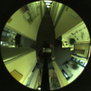
\includegraphics[width=0.15\textwidth]{cold/Saarbruecken_CR(1)}
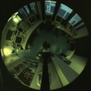
\includegraphics[width=0.15\textwidth]{cold/Saarbruecken_TR(1)}
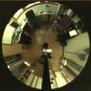
\includegraphics[width=0.15\textwidth]{cold/Freiburg_1PO(1)}
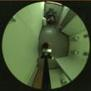
\includegraphics[width=0.15\textwidth]{cold/Freiburg_TL(1)}
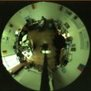
\includegraphics[width=0.15\textwidth]{cold/Ljubljana_LAB(1)}
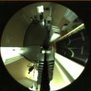
\includegraphics[width=0.15\textwidth]{cold/Ljubljana_PA(1)}
\end{center}
\caption{Sample data from the COLD database. Images were acquired from three diferent indoor laboratory enviroments located in diferent European cities: Saarbrücken, Freiburg and Ljubjlana.}
\end{figure}



Consequently, the \gls{COLD} database is an ideal testbed for assessing the robustness of localization and place recognition/categorization algorithms with respect to both categorical and dynamic changes (introduced by illumination variations and human activity).

The \gls{COLD} database is also in the process of being extend with additional data from Stockholm labs in \gls{KTH}.


\section{{ImageCLEF} - Robot Vision Task}
\subsection{History}
\gls{ImageCLEF} is the cross-language image retrieval track which is run as part of the Cross Language Evaluation Forum (CLEF). \gls{ImageCLEF} has already seen participation from both academic and commercial research groups worldwide from communities~\citep{imageclef}.
Together with each task run, datasets of training and validation data are made available providing the community with useful tools for benchmarking their methods.

It exists since 2003 and the tasks proposed by it have been evolving over-time and in 2010 it counted four main tasks: Medical Retrieval, Photo Annotation, Robot Vision and Wikipedia Retrieval.
Of which the Robot Vision is of interest to this thesis.


\subsection{Robot Vision Task in 2011}
The robot vision task~\citep{pronobis2010imageclef} which originally has been part of the \gls{ImageCLEF} since 2009 will no longer be part of it.
Nonetheless according to the organizers the competition will keep its structure and will remain active as a sole competition not part of the forum.

A transcription of the challenge description follows:

\begin{quotation}``The third edition of the challenge (2011) will focus on the problem of visual place classification, with a special focus on generalization.
Participants will be asked to classify rooms and functional areas on the basis of image sequences, captured by a stereo camera mounted on a mobile robot within an office environment.
The test sequence will be acquired within the same building but at a different floor than the training sequence.
It will contain rooms of the same categorical type ("corridor", "office", "bathroom") and it will also contain room categories not seen in the training sequence ("meeting room", "library").

The system built by participants should be able to answer the question "where are you?" when presented with a test sequence imaging a room category seen during training, and it should be able to answer "I do not know this category" when presented with a new room category.'' -- Robot Vision Task
\end{quotation}

